This section describes how the messaging system described as part of the previous chapter can be reused for the IMP solution described in this chapter.

\subsection{Integration Requirements}

Focus of the technological integration is to use the same messaging system as described in section 4.2 to integrate the new IMP solution into the different system architecture of institutions. The layout of the messaging system should not change and the purpose of each module should stay the same. In order to adapt the architecture to the new system architecture and IMP solution, the modules can be configured and named differently.

\subsection{Integration Overview}

\begin{figure}[H]
    \centering
    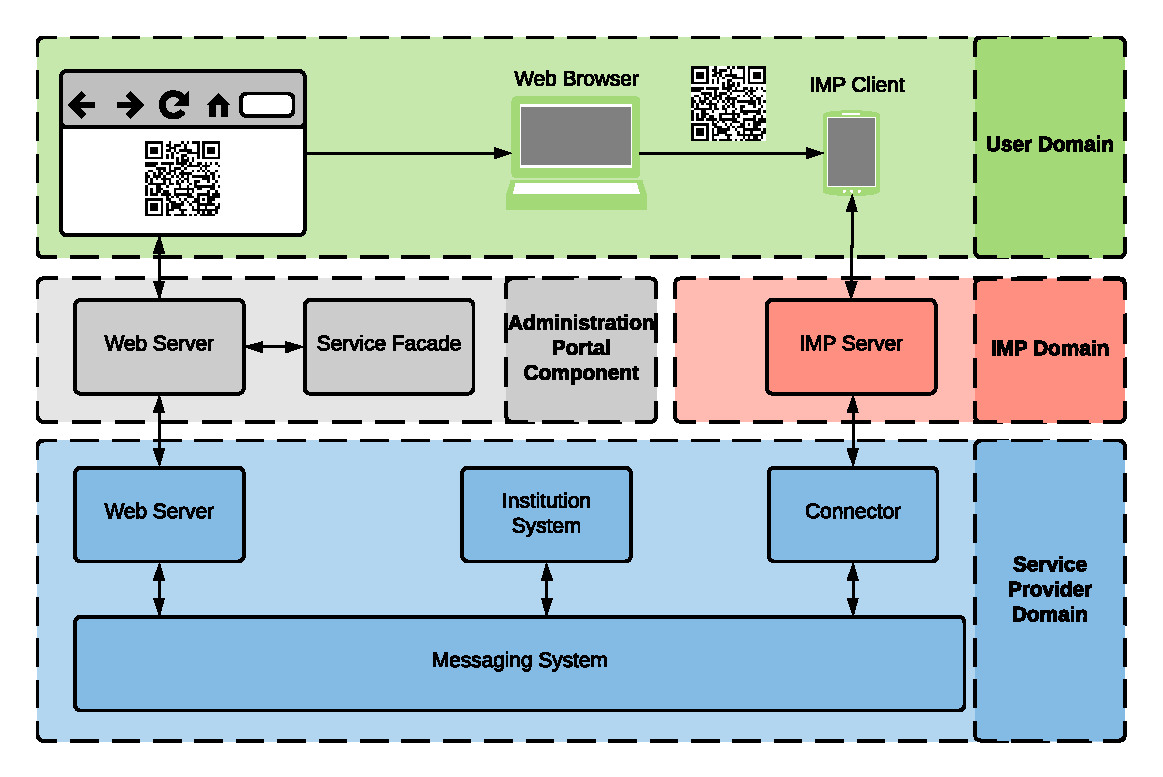
\includegraphics[scale=0.6]{Diagrams/Integration Architecture 2/Technological Integration/1. Integration Overview.pdf}
    \caption{Integration Overview}
    \label{integration2:integration_overview}
\end{figure}

To implement the IMP solution, a connector is included in the existing system architecture of each institution as well as the messaging system described in section 4.2. Instead of the web server and service facade in the portal domain, the messaging system is connected to the web server and institution system of the institution domain.

\begin{figure}[H]
    \centering
    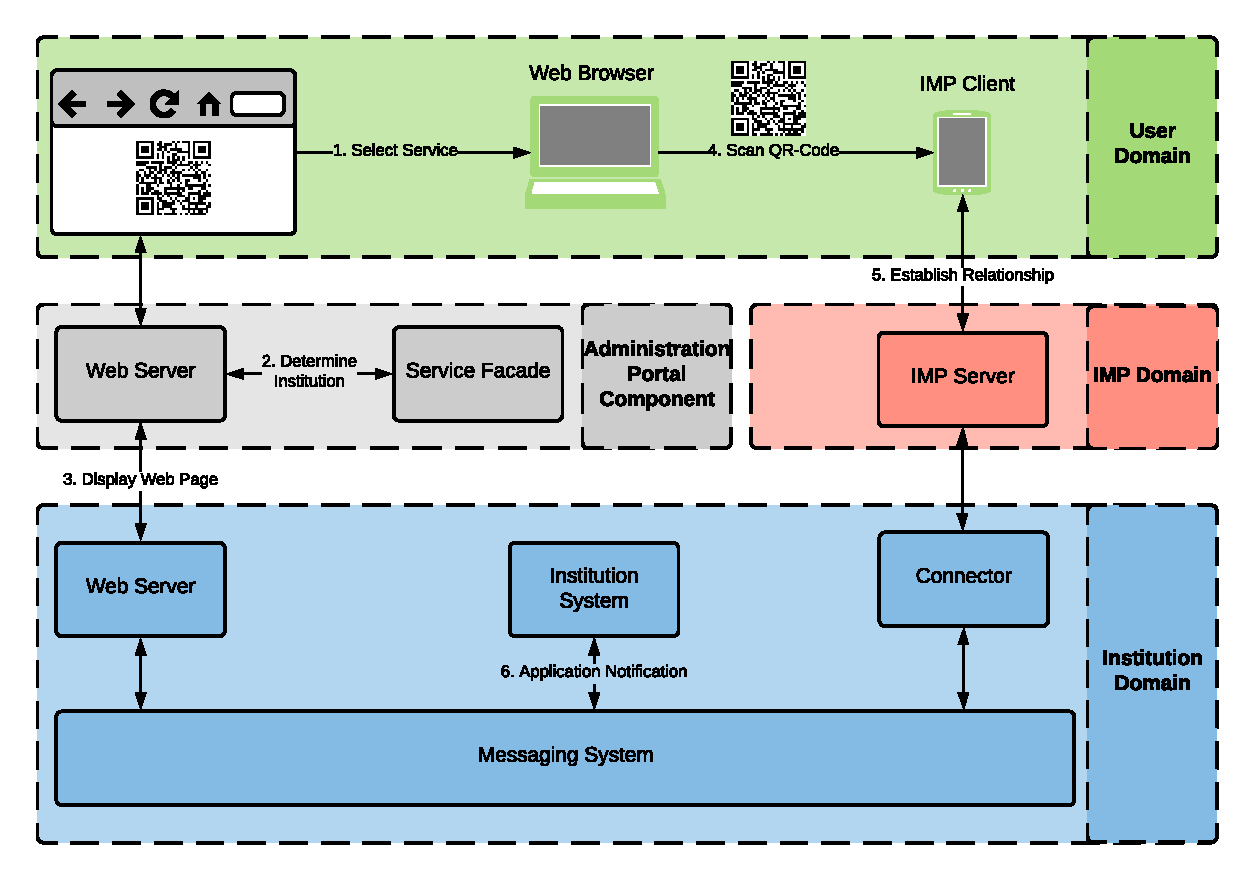
\includegraphics[scale=0.6]{Diagrams/Integration Architecture 2/Technological Integration/3. Application Overview.pdf}
    \caption{Service Application Overview}
    \label{integration2:application_overview}
\end{figure}

Institutions are able to process a predetermined set of administrative services. For each service, the institution can create a relationship template once and store it as QR code on their web page. 

Users visiting an administration portal can select an administrative service, specify their home address and be forwarded to the web page of the respective institution. After scanning the appropriate QR code with the IMP client, the user can fill in the requested attributes and send the relationship request. After the relationship is established, the institution is notified and starts processing the application utilizing the shared attributes.

\begin{figure}[H]
    \centering
    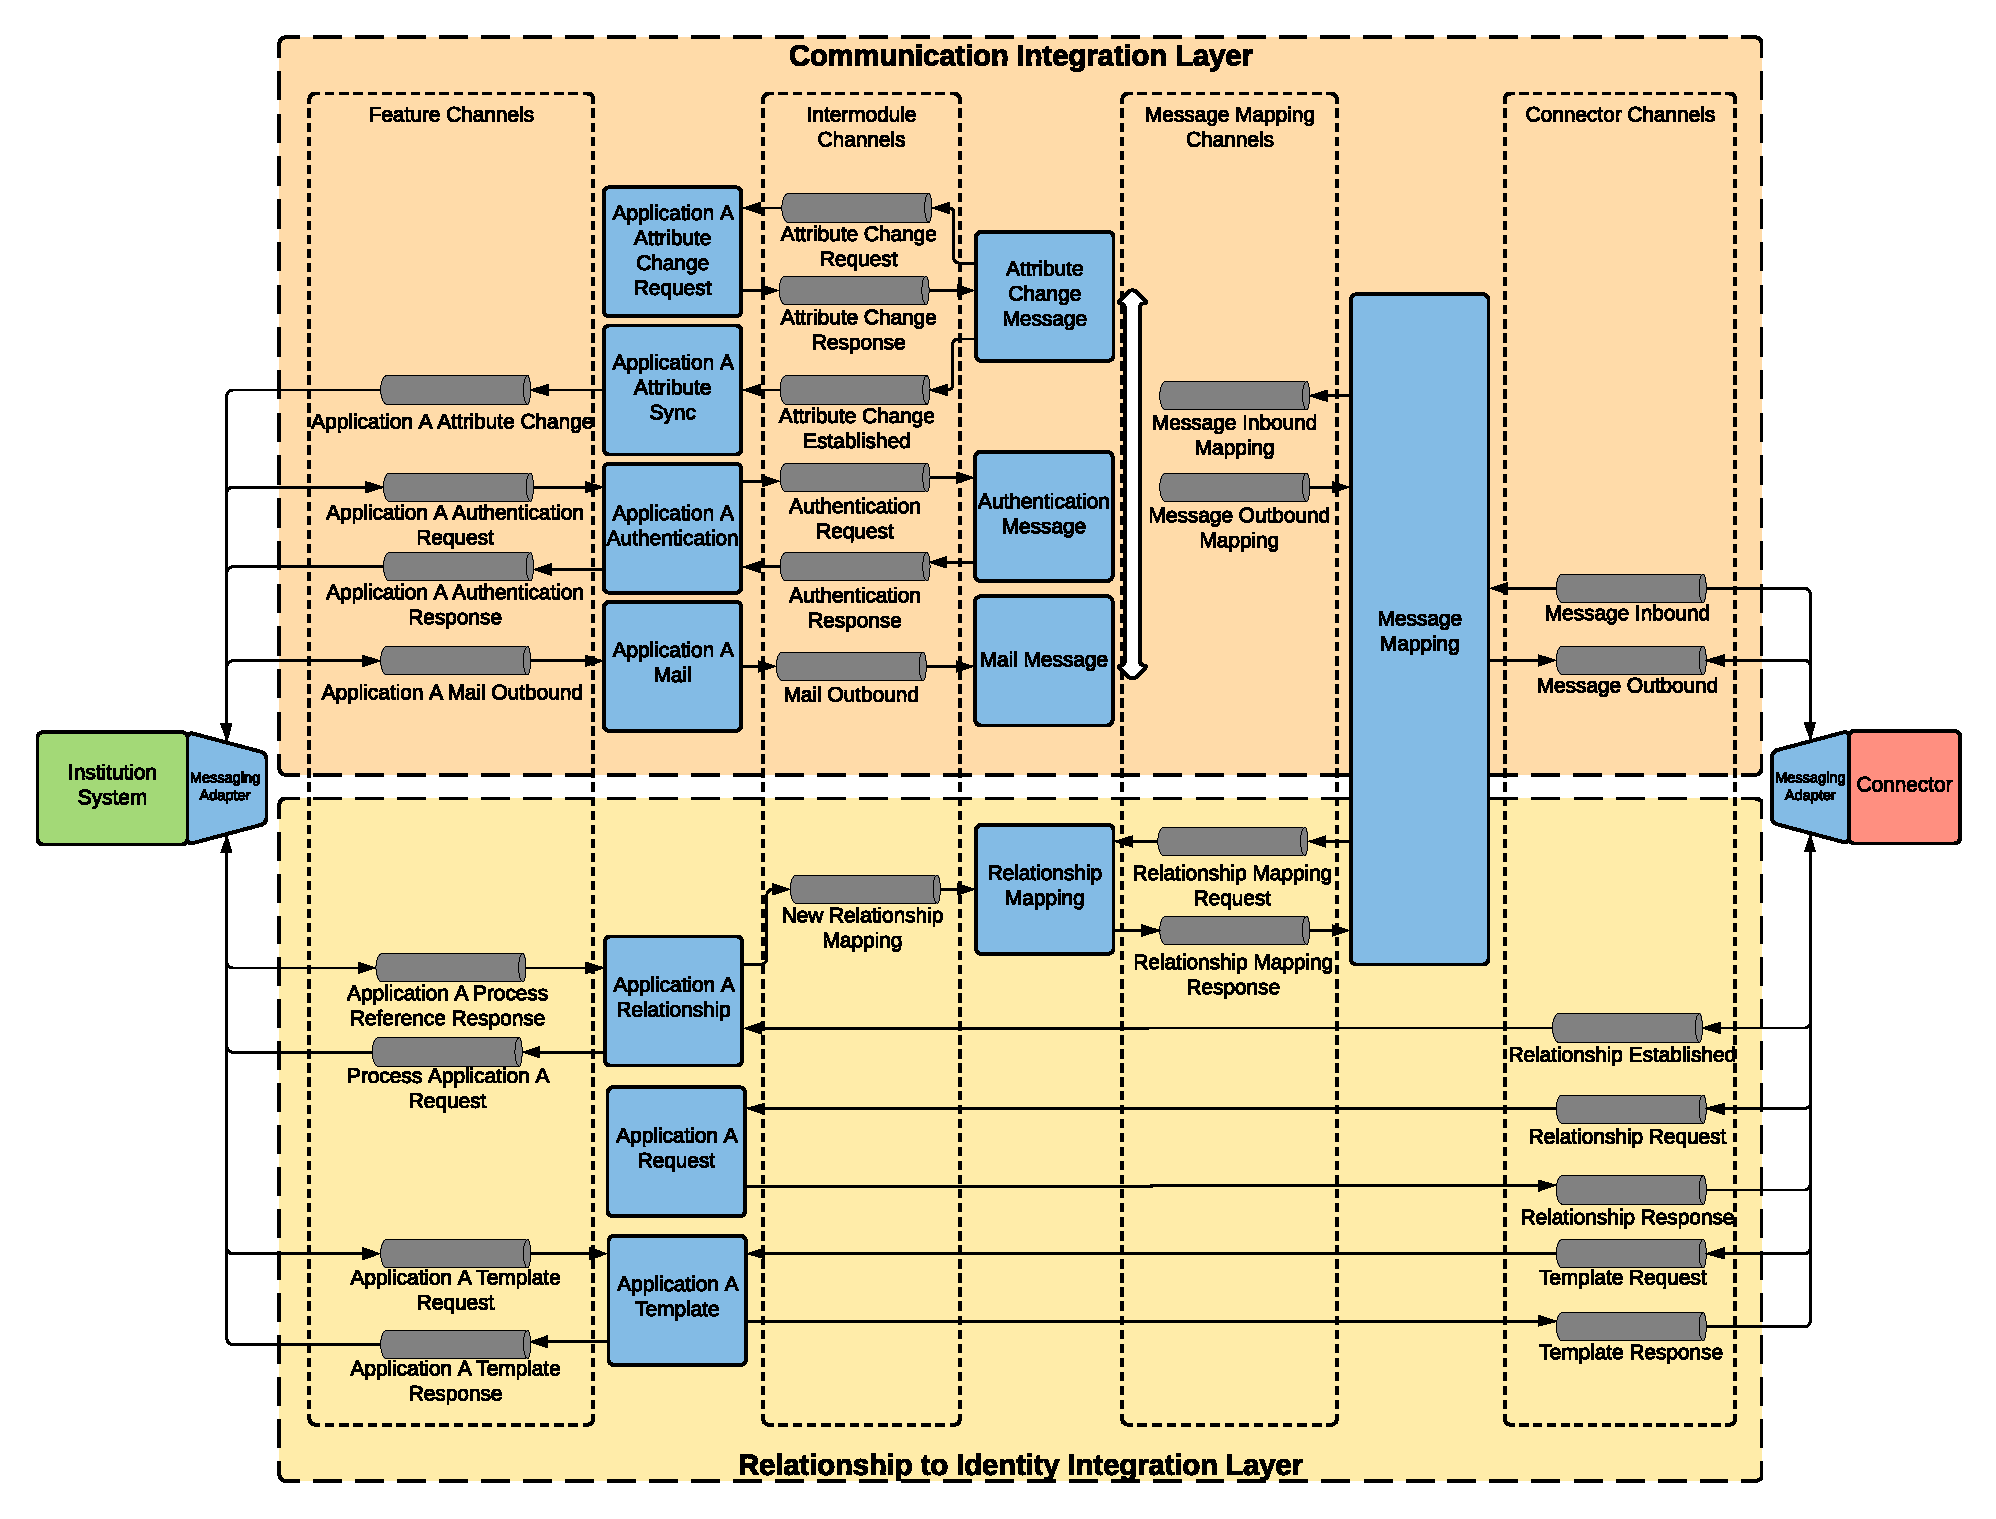
\includegraphics[scale=0.45]{Diagrams/Integration Architecture 2/Technological Integration/2. Messaging Overview.pdf}
    \caption{Messaging Overview}
    \label{integration2:messaging_overview}
\end{figure}

The layout of the messaging system is identical to the one presented in section 4.2. Exactly the same type of messages are exchanged with however a slightly different purpose and content. Therefore, in this and the following sections, only important differences between the operation of the messaging system will be described.

On the "Relationship to Identity Integration Layer", modules exist for establishing the different types of application relationships. For simplification, modules only for an "Application A" are shown. Besides the content and purpose of relationships in this case are different to the relationships of chapter 4, they are processed exactly the same: each type of relationship request is processed by an individual application request module and each type of established relationship is processed by an individual application relationship module. As the purpose of relationships in this case are applications for administrative services, each module has to be configured appropriately. For an established relationship, instead of issuing the existing system architecture to create a user profile, the application relationship module issues the existing system architecture to process an application based on the attributes shared as part of the relationship. And instead of a user profile ID, the existing system architecture responds with an application process ID. This application process ID is used in the same way as the user profile ID in section 4.2. Through the "New Relationship Mapping" channel, it is sent to the relationship mapping module, which maps each relationship to an application process and vice versa.

On the "Communication Integration Layer", the same types of messages are exchanged. However instead of user profile IDs, relationship IDs are mapped to application process IDs. In chapter 4, each module connected to the messaging adapter of the institution system was designed to be able to distinguish between different types of user profile IDs in order to for example distinguish an enterprise profile from the profile of a private person. In this case, modules can distinguish between different application types based on the application process ID.

\subsection{Messaging Modules}

\paragraph{Application Template Module}

\begin{figure}[H]
    \centering
    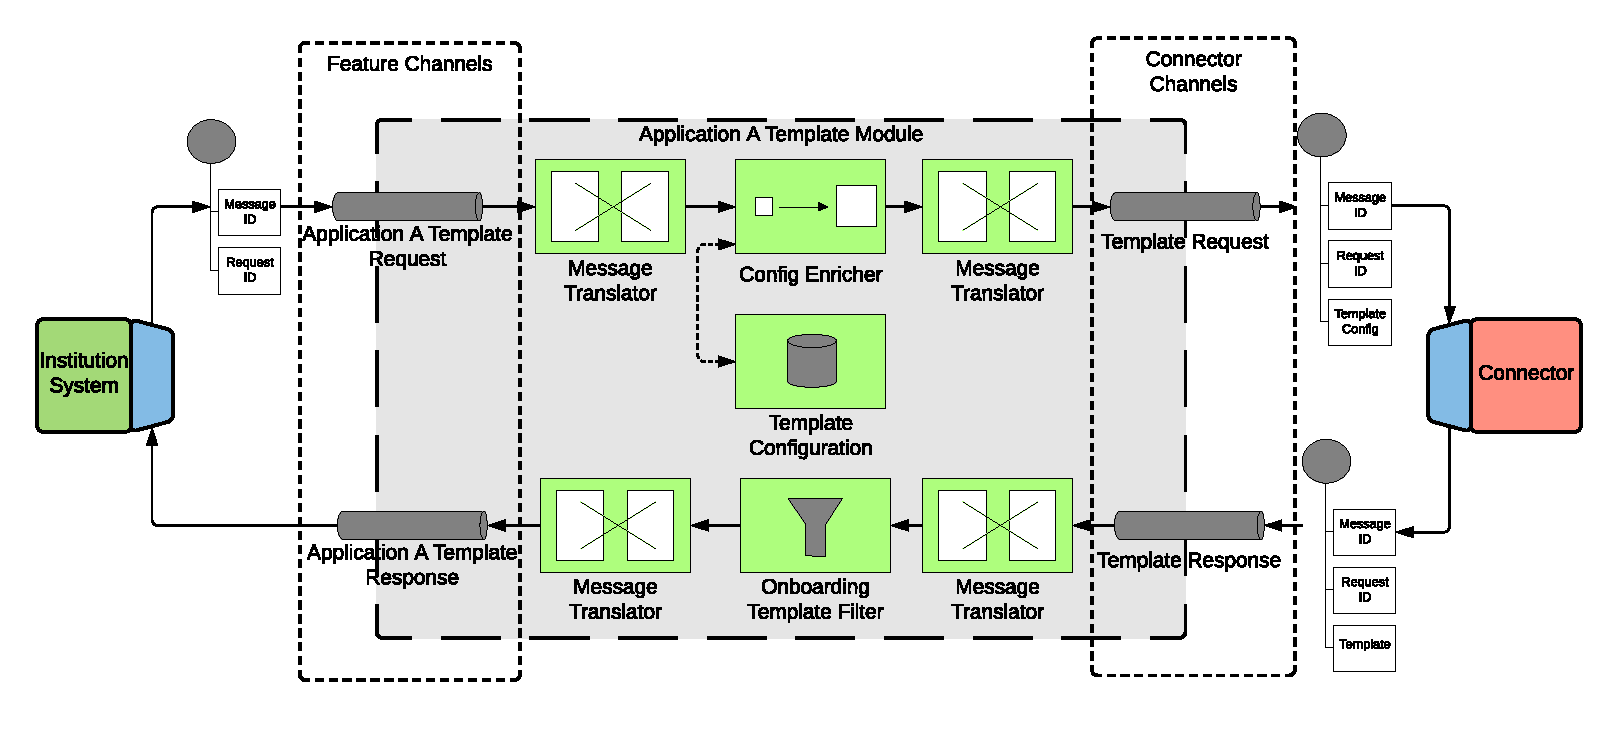
\includegraphics[scale=0.6]{Diagrams/Integration Architecture 2/Technological Integration/4. Application Template Module.pdf}
    \caption{Application Template Module}
    \label{integration2:application_template_module}
\end{figure}

Relationship templates are created manually and stored as a QR-code image on the web page of the institution. For each application type, a separate application template module can be included which stores the configuration for the template type and issues the connector to create new relationship templates. Instead of the web page, the institution system is connected, as application templates are not dynamically created for user requests but once by an employee of the institution. Each time the content of an application template has to be changed, the institution creates a new one through this module.

\paragraph{Application Request Module}

\begin{figure}[H]
    \centering
    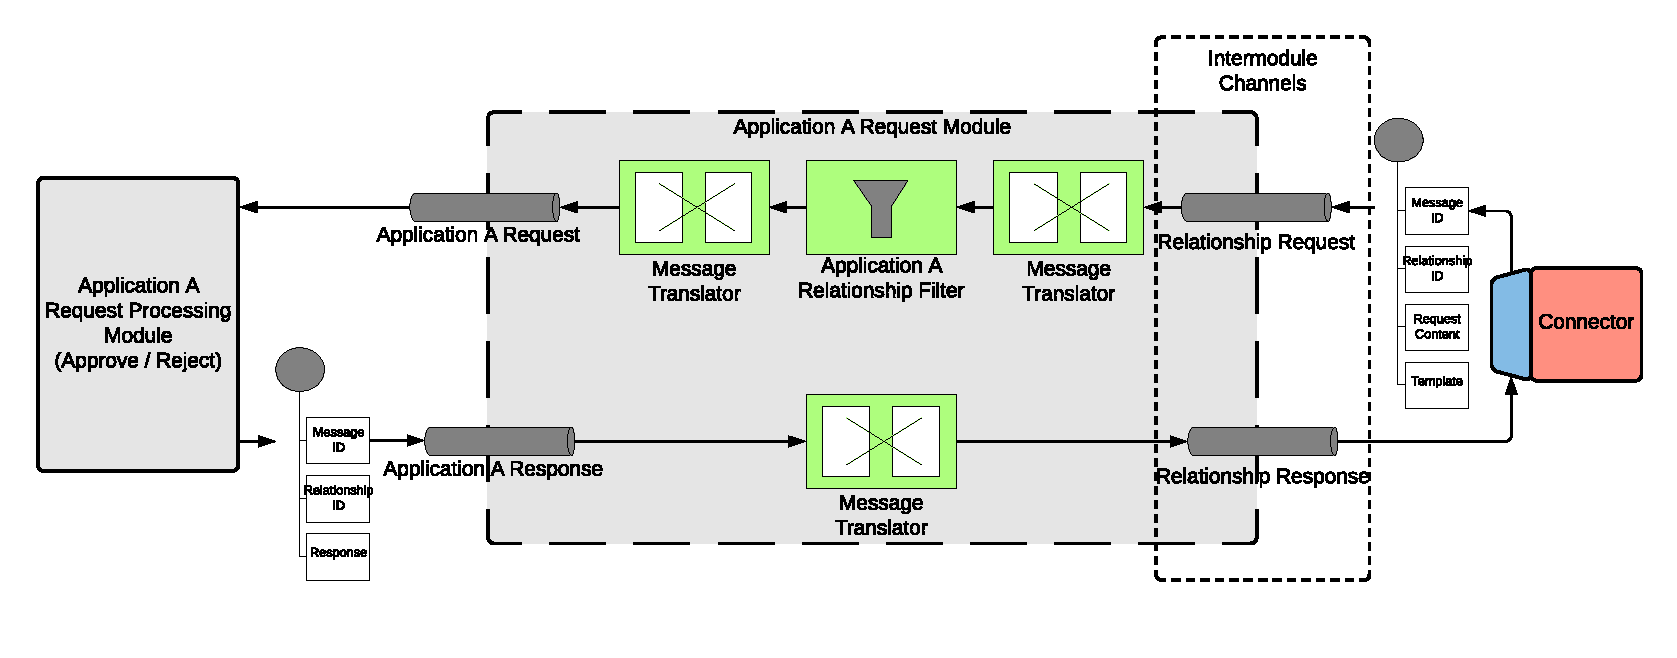
\includegraphics[scale=0.6]{Diagrams/Integration Architecture 2/Technological Integration/5. Application Request Module.pdf}
    \caption{Application Request Module}
    \label{integration2:application_request_module}
\end{figure}

For each type of application relationship, a different application request module is used to separate the processing of requests for different application types into application request processing modules. Depending on the type of application, different requirements regarding the acceptance of application requests exist. A request processing module might for example check if the home address of the user is within the are of responsibility of the institution. Only after the relationship and therefore the application request is accepted the application will be processed.

\paragraph{Application Relationship Module}

\begin{figure}[H]
    \centering
    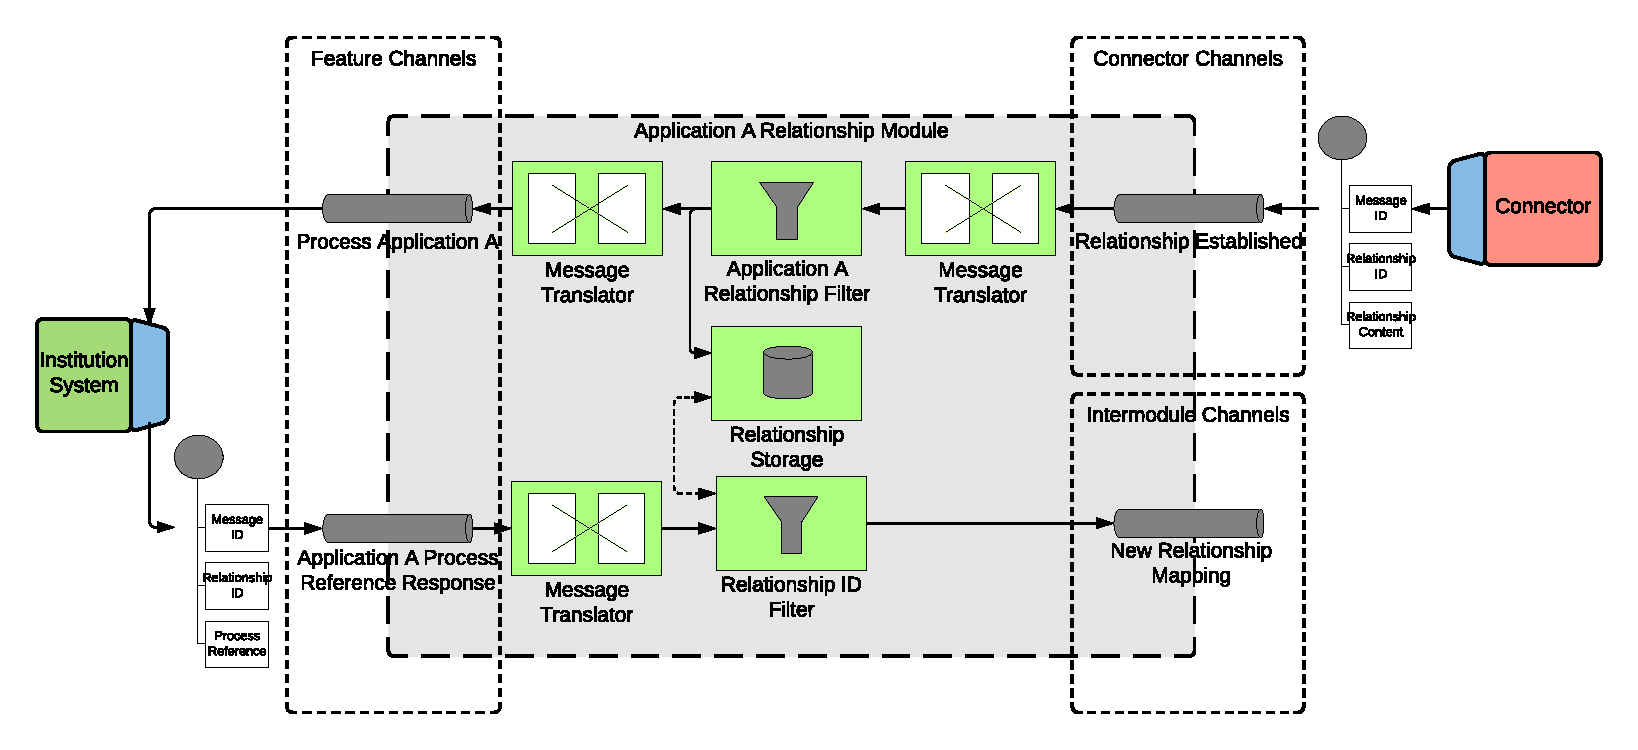
\includegraphics[scale=0.6]{Diagrams/Integration Architecture 2/Technological Integration/6. Application Relationship Module.pdf}
    \caption{Application Relationship Module}
    \label{integration2:application_relationship_module}
\end{figure}

For each type of application relationship a different application relationship module is used for processing established relationships. The institution system is notified of an accepted application through the "Process Application Request" channel. As part of the existing system architecture, institution systems received applications through the data exchange platform as an application document. In order to adhere to this standard, the message translator connected to the "Process Application Request" channel translates the relationship content into the application format of documents delivered through the data exchange platform. As explained in section 2.3.2, form servers create the application documents based on a standard defined by FIM.

Institution systems are assumed to uniquely reference active applications with process IDs. After starting the application process, the institution responds through the messaging adapter with the process ID on the "Application Process Reference Response" channel. This process ID is then published on the "New Relationship Mapping" channel. The result is, that in contrast to the messaging system of chapter 4, relationships are not mapped to user profiles but to application processes.

\paragraph{Application Attribute Change Request Module}

\begin{figure}[H]
    \centering
    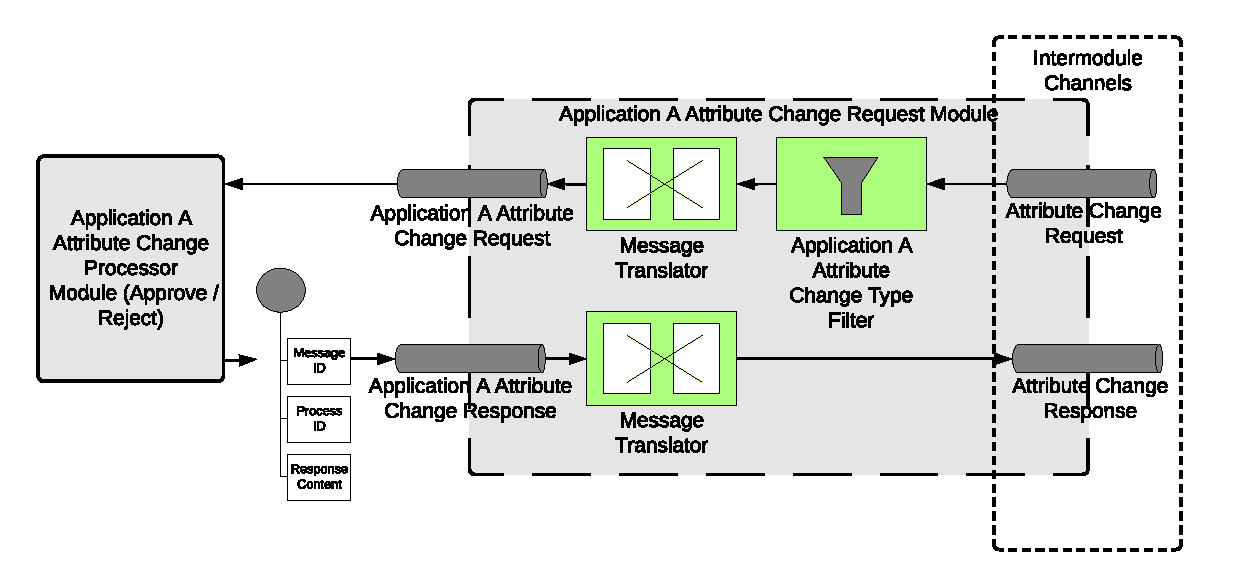
\includegraphics[scale=0.6]{Diagrams/Integration Architecture 2/Technological Integration/7. Application Attribute Change Request Module.pdf}
    \caption{Application Attribute Change Request Module}
    \label{integration2:application_attribute_change_request_module}
\end{figure}

As an example for a message type processed on the "Communication Integration Layer", the application attribute change messages are selected.

In the same way as in chapter 4, attribute change message types are published on individual channels, this time however, instead of a user profile ID, they contain a process ID. As described on the example of different user profile ID types in chapter 4, different process ID types may exist in this case too. For example, an attribute change request for an application of type "A" might be processed differently to an attribute change request for an application of type "B". To process different types of attribute change requests separately, multiple application attribute change request modules can be included, each of them filtering for different types of process IDs. If it is possible to retrieve the application type from the process ID, processing of each application type could be separated into multiple application change request modules. In case application types are not retrievable from process IDs, an additional module can be included, which requests the application type from the institution system based on the process ID. An alternative would be for the application relationship module to not only publish the process ID corresponding to a relationship ID on the "New Relationship Mapping" channel but also the application type.

Only after the attribute change request is accepted, the institution system will be notified about the attribute change.

\paragraph{Application Attribute Sync Module}

Continuing the example of how application attribute change messages are processed on the "Communication Integration Layer", the application attribute sync module processes messages on the "Attribute Change Established" channel. With the same reasoning as in the previous section, the message filter attached to the channel enables to include multiple application attribute sync modules, processing different application types.

The institution system receives the notification from the application through the messaging adapter. Depending on the capabilities of the institution system, this could result in either an automated update of the referenced application process or an automated e-mail to the assigned employee.

\paragraph{Application Mail Module}

Similar to the attribute change messages, mail messages can be fitted to the process based scenario, enabling institutions to send mails to a process ID which the messaging system translates to a relationship ID in order for the correct IMP identity to receive it. In addition to the one directional message transfer from the institution to the IMP identity, the application mail module and the mail message module could be expanded to be able to receive mails from an IMP identity through an established relationship. The relationship ID of the message would be mapped to the corresponding process ID and submitted to the institution system. The institution system could then send the mail to the responsible employee.

\paragraph{Application Authentication Module}

Authentication messages and modules are not required for this IMP solution, as no user profile and therefore no login process exists. However, depending on the use case, authentication messages could be included as an additional accept / reject communication method between institution and user.

\subsection{Evaluation}
The integration architecture enables users to directly interact with the system architecture of the Service Provider for submitting applications. This eliminates the need for administration portals to process personal information.

\begin{figure}[h]
    \centering
    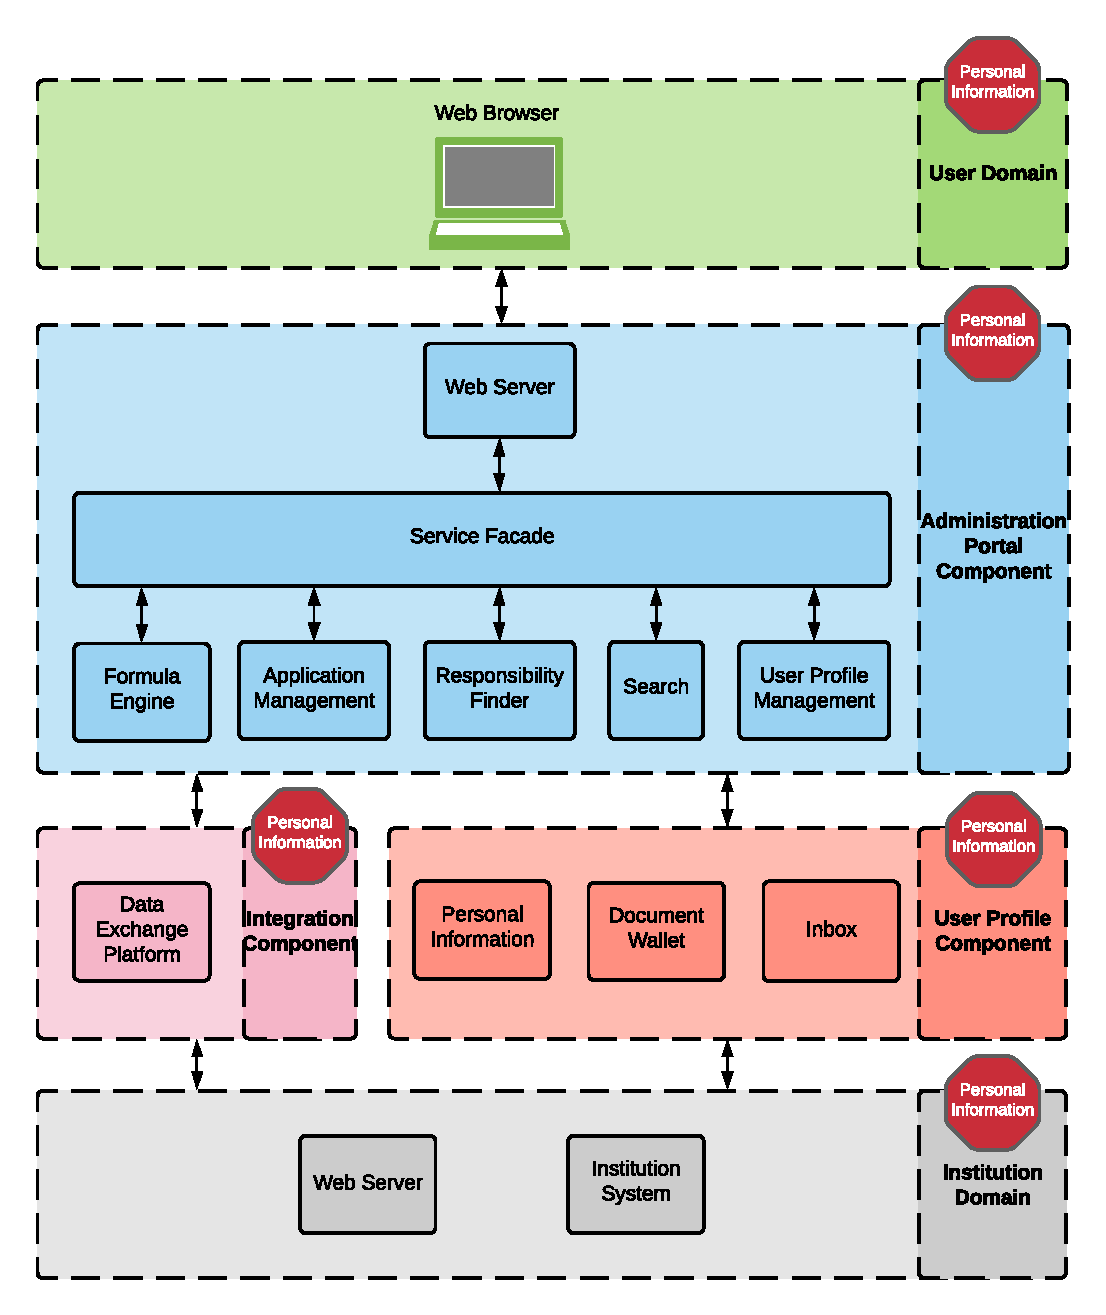
\includegraphics[scale=0.6]{Diagrams/Integration Architecture 2/OZG Personal Information.pdf}
    \caption{OZG System Architecture Personal Information}
    \label{integration2:ozg_personal_information}
\end{figure}

\begin{figure}[h]
    \centering
    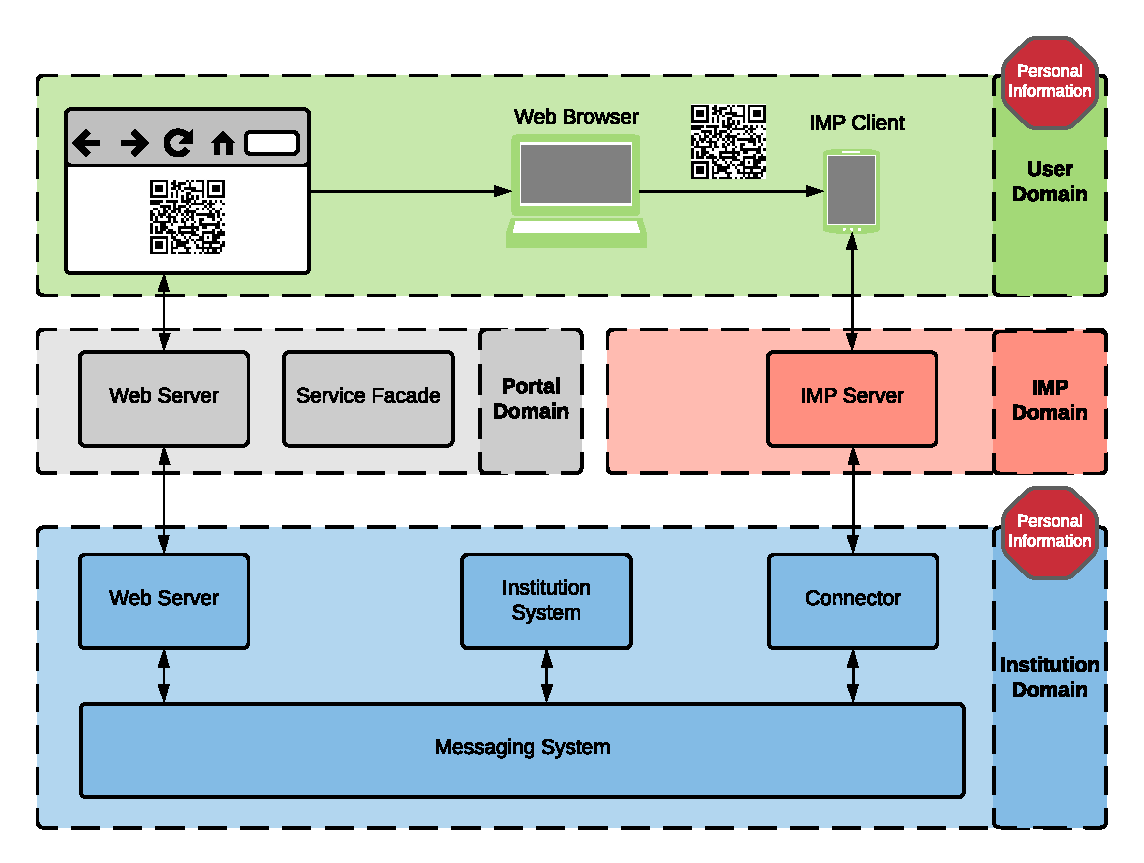
\includegraphics[scale=0.6]{Diagrams/Integration Architecture 2/IMP Personal Information.pdf}
    \caption{IMP System Architecture Personal Information}
    \label{integration2:imp_personal_information}
\end{figure}

Comparing the existing system architecture of the OZG with the system architecture utilizing IMP, the amount of systems processing personal information is reduced. Using this IMP solution, only the user and the responsible institution have access to personal information.

The integration architecture described in section 4.2 was able to integrate into two different system architectures. This demonstrates, that the presented integration architecture is applicable to a variety of system architectures.

It was also able to integrate a user oriented (persistent) relationship scenario as well as a process oriented (temporary) relationship scenario. This demonstrates that the presented integration architecture can be used for integrating a variety of IMP solutions.

The modular message based approach made it possible to use the integration architecture in a different scenarios, by enabling easy configuration of modules for new requirements.
